\documentclass[tikz,border=8pt]{standalone}
\usepackage[utf8]{inputenc}
\usepackage{lmodern}
\usepackage[T1]{fontenc}
\usepackage{amsmath,amssymb}
\usetikzlibrary{shapes.geometric, arrows.meta, positioning, calc, fit, backgrounds}

\definecolor{greenA}{HTML}{15803D}
\definecolor{greenB}{HTML}{22C55E}
\definecolor{greenC}{HTML}{F0FDF4}
\definecolor{skyA}{HTML}{0369A1}
\definecolor{skyB}{HTML}{38BDF8}
\definecolor{skyC}{HTML}{F0F9FF}
\definecolor{fuchsiaA}{HTML}{A21CAF}
\definecolor{fuchsiaC}{HTML}{FDF4FF}
\definecolor{slateG}{HTML}{475569}
\definecolor{amberA}{HTML}{D97706}
\definecolor{amberC}{HTML}{FEF3C7}

\begin{document}
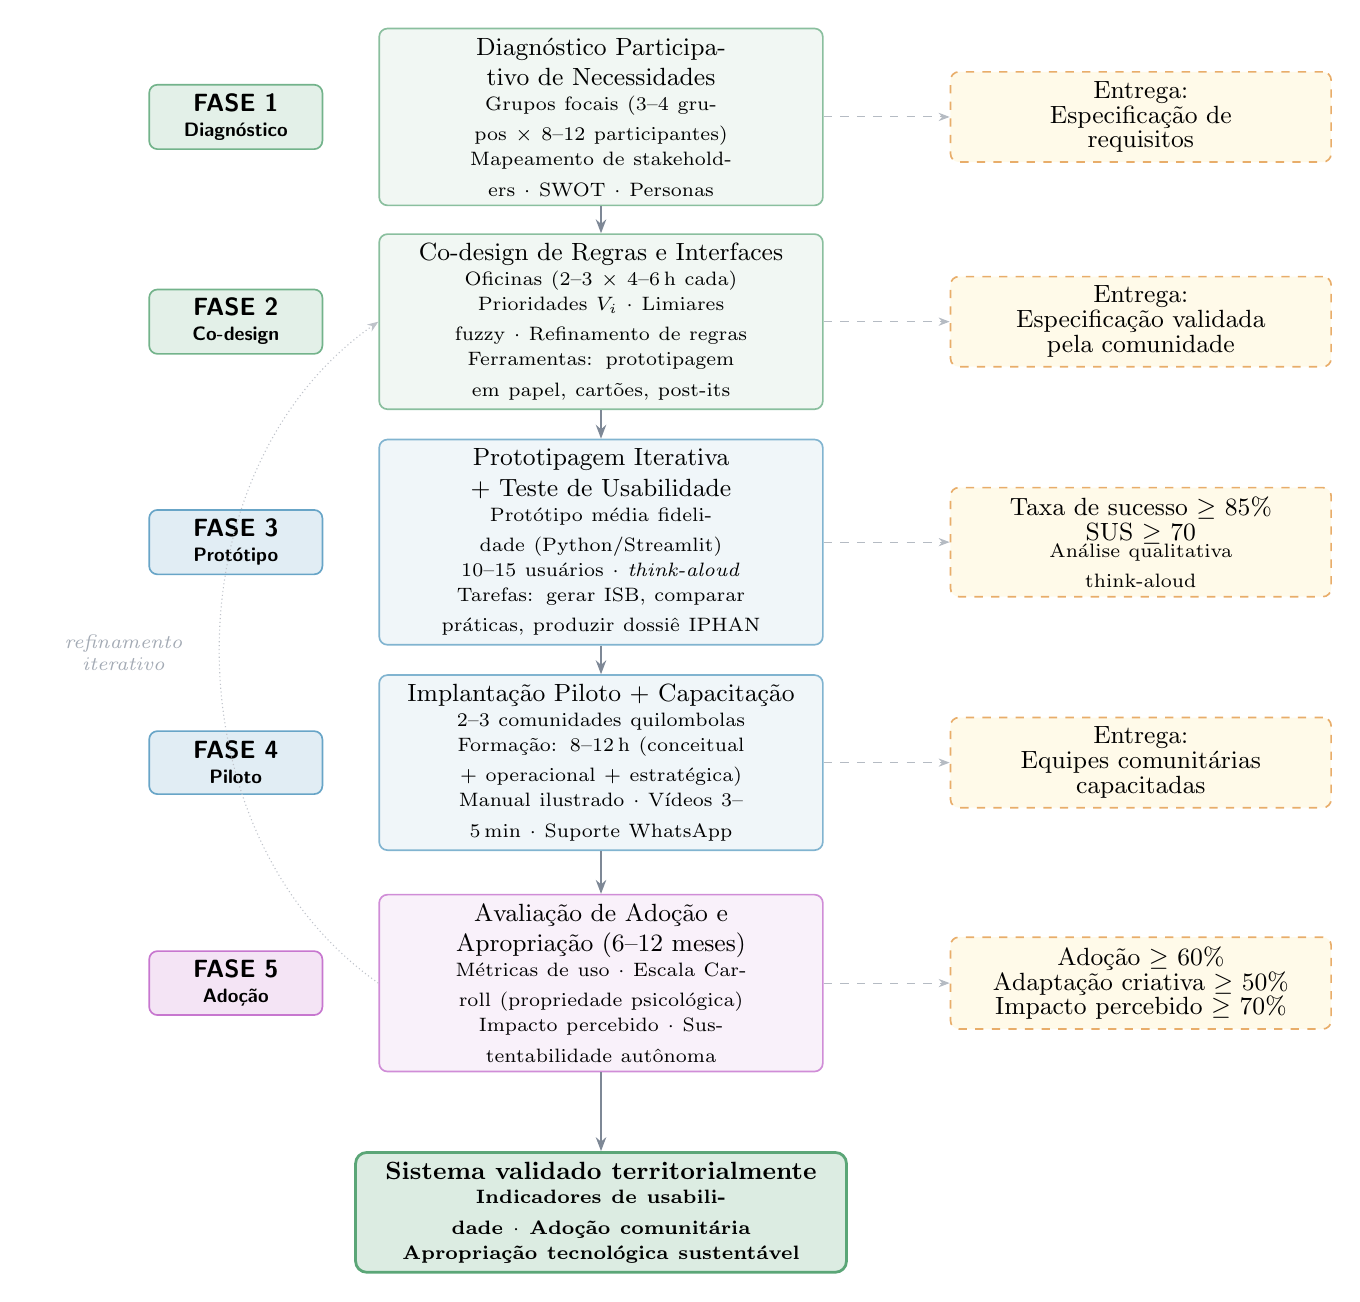
\begin{tikzpicture}[
  phase/.style={
    fill=#1!12, draw=#1!60,
    font=\sffamily\bfseries\small,
    minimum width=2.2cm, minimum height=0.8cm,
    align=center, rounded corners=3pt,
    line width=0.6pt
  },
  stepbox/.style={
    draw=#1!50, fill=#1!6,
    font=\small, align=center,
    minimum width=5.6cm, minimum height=0.9cm,
    rounded corners=3pt, text width=5.4cm,
    line width=0.6pt
  },
  metricbox/.style={
    draw=amberA!60, fill=amberC!40,
    font=\small, align=center,
    minimum width=4.8cm, minimum height=0.9cm,
    rounded corners=3pt, text width=4.6cm,
    line width=0.6pt, dashed
  },
  outputbox/.style={
    draw=#1!70, fill=#1!15,
    font=\small\bfseries, align=center,
    minimum width=6.2cm, minimum height=1.0cm,
    rounded corners=4pt, text width=6.0cm,
    line width=1pt
  },
  arr/.style={-{Stealth[length=5pt]}, thick, slateG!70},
  darr/.style={-{Stealth[length=4pt]}, thin, slateG!40, dashed},
  feedback/.style={-{Stealth[length=4pt]}, thin, slateG!35, densely dotted},
]

%% ═══ FASE 1 — DIAGNÓSTICO PARTICIPATIVO ═══
\node[phase=greenA] (ph1) at (0,0) {FASE 1\\[-2pt]{\scriptsize Diagn\'ostico}};

\node[stepbox=greenA, right=0.7cm of ph1] (f1)
  {Diagn\'ostico Participativo de Necessidades\\[-2pt]
   {\scriptsize Grupos focais (3--4 grupos $\times$ 8--12 participantes)}\\[-2pt]
   {\scriptsize Mapeamento de stakeholders $\cdot$ SWOT $\cdot$ Personas}};

\node[metricbox, right=1.6cm of f1] (m1)
  {Entrega:\\[-2pt]
   Especifica\c{c}\~ao de\\[-2pt]
   requisitos};
\draw[darr] (f1) -- (m1);

%% ═══ FASE 2 — CO-DESIGN ═══
\node[phase=greenA] (ph2) at (0,-2.6) {FASE 2\\[-2pt]{\scriptsize Co-design}};

\node[stepbox=greenA, right=0.7cm of ph2] (f2)
  {Co-design de Regras e Interfaces\\[-2pt]
   {\scriptsize Oficinas (2--3 $\times$ 4--6\,h cada)}\\[-2pt]
   {\scriptsize Prioridades $V_i$ $\cdot$ Limiares fuzzy $\cdot$ Refinamento de regras}\\[-2pt]
   {\scriptsize Ferramentas: prototipagem em papel, cart\~oes, post-its}};
\draw[arr] (f1.south) -- (f2.north);

\node[metricbox, right=1.6cm of f2] (m2)
  {Entrega:\\[-2pt]
   Especifica\c{c}\~ao validada\\[-2pt]
   pela comunidade};
\draw[darr] (f2) -- (m2);

%% ═══ FASE 3 — PROTOTIPAGEM + USABILIDADE ═══
\node[phase=skyA] (ph3) at (0,-5.4) {FASE 3\\[-2pt]{\scriptsize Prot\'otipo}};

\node[stepbox=skyA, right=0.7cm of ph3] (f3)
  {Prototipagem Iterativa + Teste de Usabilidade\\[-2pt]
   {\scriptsize Prot\'otipo m\'edia fidelidade (Python/Streamlit)}\\[-2pt]
   {\scriptsize 10--15 usu\'arios $\cdot$ \textit{think-aloud}}\\[-2pt]
   {\scriptsize Tarefas: gerar ISB, comparar pr\'aticas, produzir dossi\^e IPHAN}};
\draw[arr] (f2.south) -- (f3.north);

\node[metricbox, right=1.6cm of f3] (m3)
  {Taxa de sucesso $\geq$ 85\%\\[-2pt]
   SUS $\geq$ 70\\[-2pt]
   {\scriptsize An\'alise qualitativa\\think-aloud}};
\draw[darr] (f3) -- (m3);

%% ═══ FASE 4 — IMPLANTAÇÃO PILOTO ═══
\node[phase=skyA] (ph4) at (0,-8.2) {FASE 4\\[-2pt]{\scriptsize Piloto}};

\node[stepbox=skyA, right=0.7cm of ph4] (f4)
  {Implanta\c{c}\~ao Piloto + Capacita\c{c}\~ao\\[-2pt]
   {\scriptsize 2--3 comunidades quilombolas}\\[-2pt]
   {\scriptsize Forma\c{c}\~ao: 8--12\,h (conceitual + operacional + estrat\'egica)}\\[-2pt]
   {\scriptsize Manual ilustrado $\cdot$ V\'{\i}deos 3--5\,min $\cdot$ Suporte WhatsApp}};
\draw[arr] (f3.south) -- (f4.north);

\node[metricbox, right=1.6cm of f4] (m4)
  {Entrega:\\[-2pt]
   Equipes comunit\'arias\\[-2pt]
   capacitadas};
\draw[darr] (f4) -- (m4);

%% ═══ FASE 5 — AVALIAÇÃO DE ADOÇÃO ═══
\node[phase=fuchsiaA] (ph5) at (0,-11.0) {FASE 5\\[-2pt]{\scriptsize Ado\c{c}\~ao}};

\node[stepbox=fuchsiaA, right=0.7cm of ph5] (f5)
  {Avalia\c{c}\~ao de Ado\c{c}\~ao e Apropria\c{c}\~ao (6--12 meses)\\[-2pt]
   {\scriptsize M\'etricas de uso $\cdot$ Escala Carroll (propriedade psicol\'ogica)}\\[-2pt]
   {\scriptsize Impacto percebido $\cdot$ Sustentabilidade aut\^onoma}};
\draw[arr] (f4.south) -- (f5.north);

\node[metricbox, right=1.6cm of f5] (m5)
  {Ado\c{c}\~ao $\geq$ 60\%\\[-2pt]
   Adapta\c{c}\~ao criativa $\geq$ 50\%\\[-2pt]
   Impacto percebido $\geq$ 70\%};
\draw[darr] (f5) -- (m5);

%% ═══ SAÍDA ═══
\node[outputbox=greenA, below=1.0cm of f5] (out)
  {Sistema validado territorialmente\\[-2pt]
   {\scriptsize Indicadores de usabilidade $\cdot$ Ado\c{c}\~ao comunit\'aria}\\[-2pt]
   {\scriptsize Apropria\c{c}\~ao tecnol\'ogica sustent\'avel}};
\draw[arr] (f5) -- (out);

%% ═══ RETROALIMENTAÇÃO ═══
\draw[feedback, bend left=55] (f5.west) to
  node[left, font=\scriptsize\itshape, text=slateG!50, text width=2.2cm, align=center]
  {refinamento\\iterativo}
  (f2.west);

\end{tikzpicture}
\end{document}
